%!TEX encoding = UTF-8 Unicode
\chapter{Aspekte}
Aspekte Aspekte
\section{Markt}
	\subsection{Markt für IT-Consulting}
	In den letzten Jahren ist der Markt für Beratungsleistungen in Deutschland stark gewachsen. Während im Jahr 1992 noch 5,9 Mrd.\texteuro Umsatz für Beratungsleistungen erzielt wurden(Quelle: BDU 2003), waren es im Jahr 2008 bereits 18,2 Mrd. \texteuro (Quelle:BDU 2009) und im Jahr 2012 betrug der Umsatz schon 22,30 Mrd. \texteuro (Abb.1).
\begin{figure}[htp]
\centering
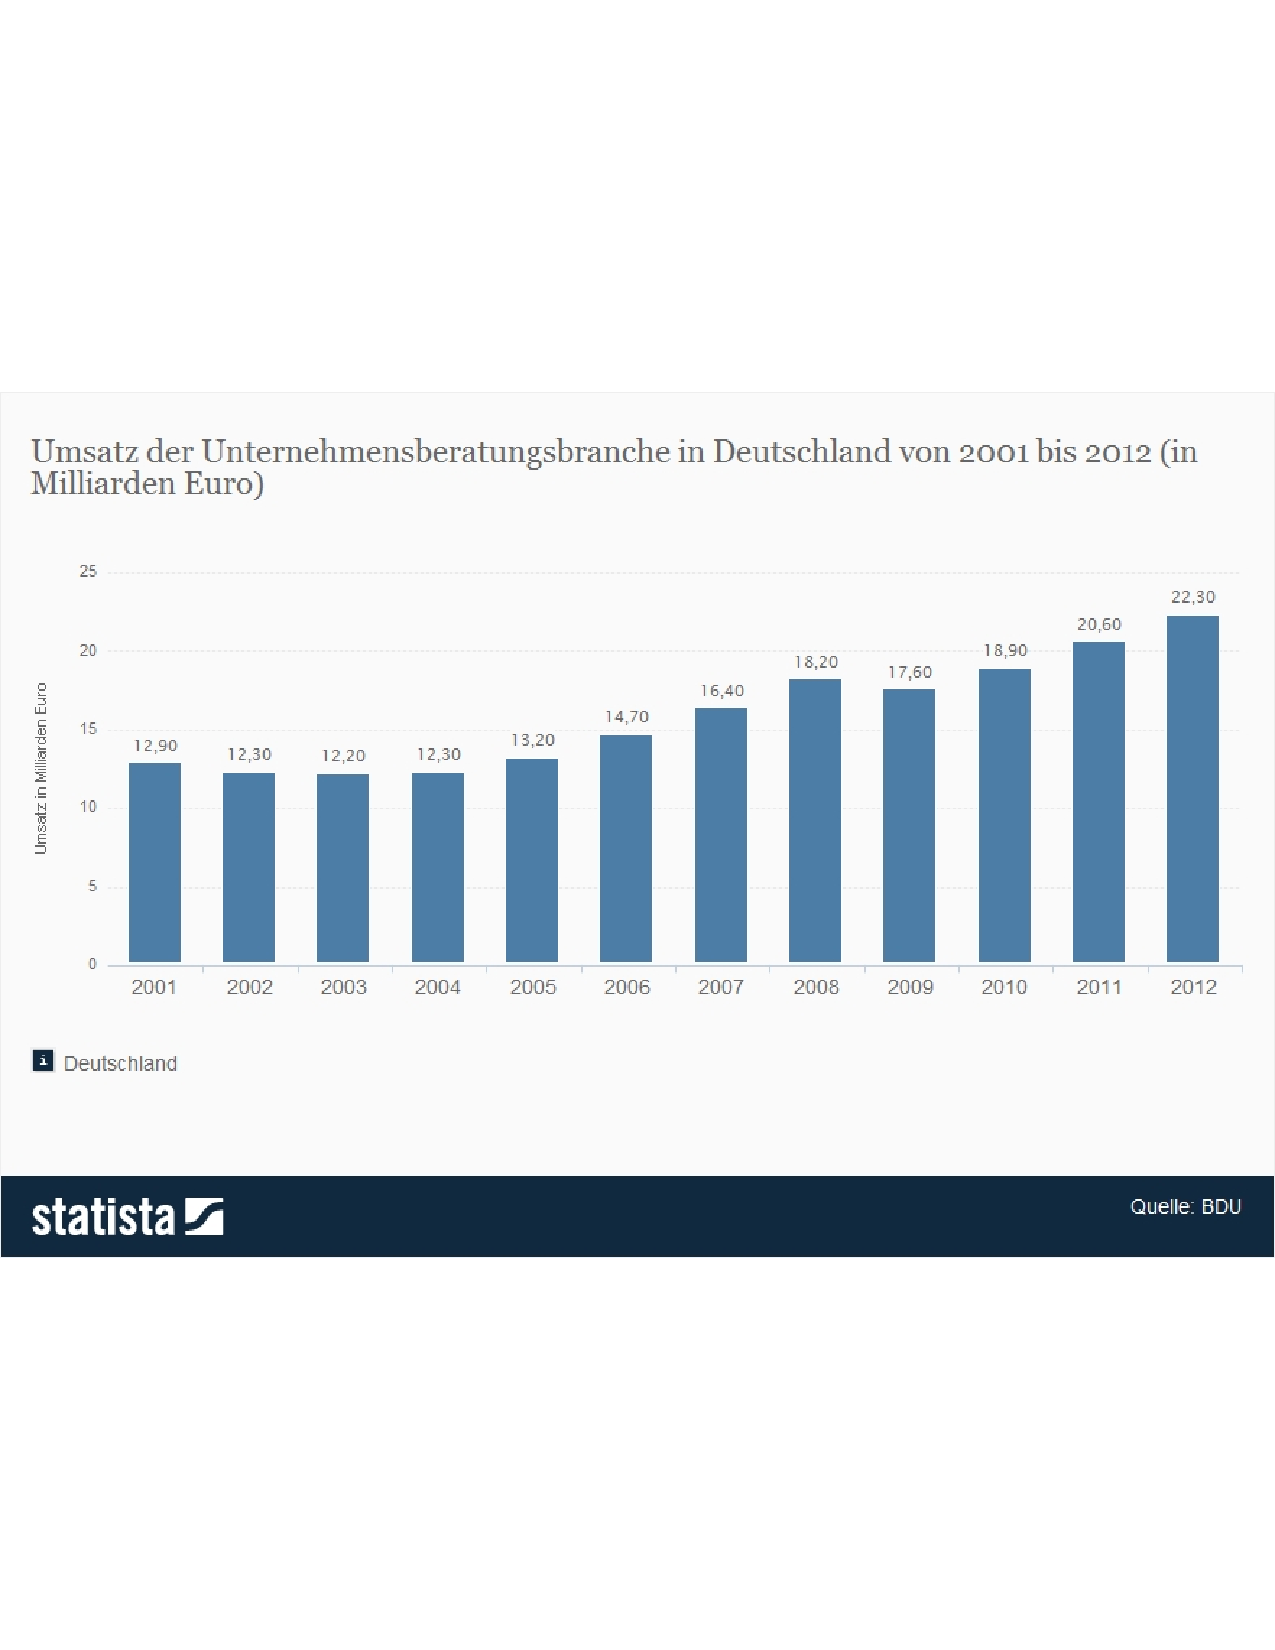
\includegraphics[width=7 cm]{images/UmsatzUBeratungsbrancheDeutschland.pdf}
\end{figure}
\section{Arbeitskultur}
	\subsection{Einleitung Arbeitskultur}
Arbeitskultur ist ....
Arbeitskultur ist eine Teilmenge der Kultur(Sitten,Bräuche) einer Nation. Sie gehört zum Beratungsprozess und spielt dabei nicht die unwesentlichste Rolle. IT-Consultans kennen innerhalb der wenigsten Zeit sehr viele Firmen und deren Mitarbeiter kennen. Berater arbeiten öfter durch Iteration mit Menschen:\\
1)aus unterschiedlichen Unternehmensebenen, angefangen von normalen Mitarbeiter(Interaktion mit Beratern während den Schulungsmaßnahmen bei IT-Neueinführung) bis zu Top-Managementebenen(Interaktion mit Beratern während der strategischen Fragen wie Planung von Anwendungssoftware, Analyse von Geschäftsprozessen usw.)\\
2)aus verschiedenen Branchen wie Finanzdienstleistung,Fahrzeugbau, Großhandel usw(Abb.2).

\begin{figure}[htp]
\centering
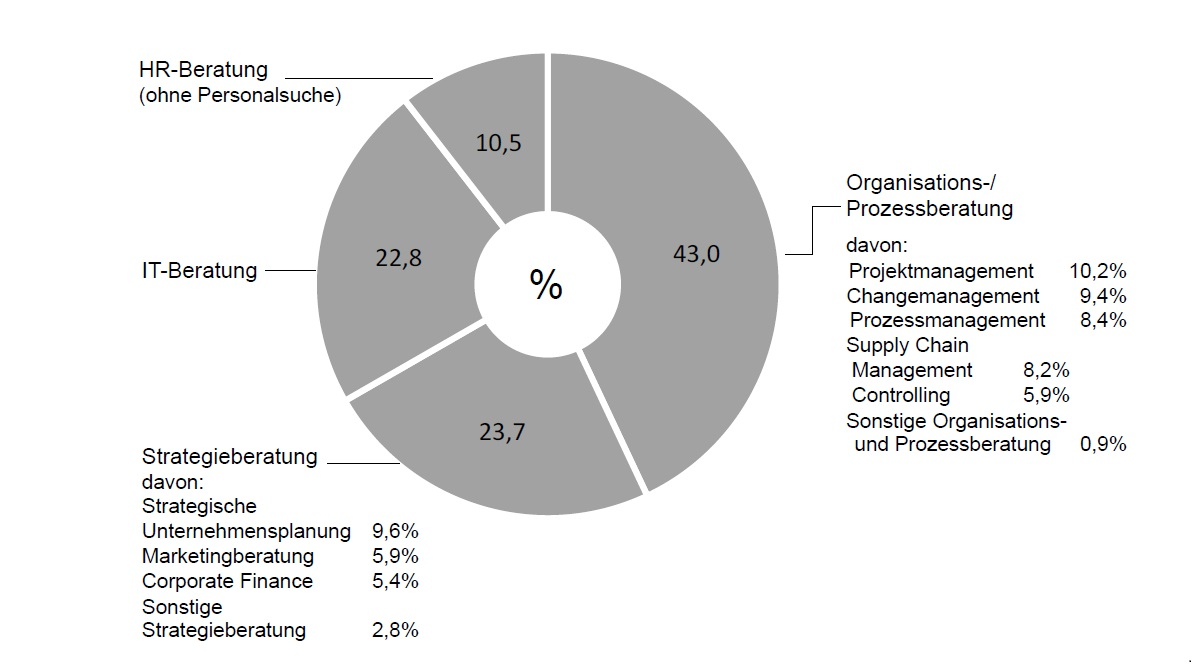
\includegraphics[width=12 cm]{images/struktur_ber_markt.pdf}
\end{figure}
Abb.2 Aufteilung des Gesamtmarktes für Unternehmensberatung\\
\\
3)aus unterschiedlichen Länder mit jeweils eigenartigen Kulturen.\\
 In diesem Punkt werden 2 Standardfälle erläutert um die Bedeutung der Arbeitskultur im Beratungsprozess zu zeigen.\\
 a) Das erste Fall ist ein IT-Consulting Unternehmen mit Beratern die aus unterschiedlichen Ländern kommen, die unterschiedliche Sprache sprechen und sich kulturell enorm unterscheiden.Diese Berater arbeiten zielgerichtet und ständig im Team. In diesem Fall wird dem Author dieser Arbeit sehr interessant inwieweit sich kulturelle Unterschiede auf das gemeinsame Ziel des Beratungsprozesses bei der Softwareeinführung auswirken können. Auch interessant ist hier wie die IT-Berater aus unterschiedlichen Länder mit Kunden aus Deutschland umgehen, ob die kulturelle Unterschiede einen Einfluss auf Kundenbeziehungen haben oder nicht. \\
 b) Das 2. Fall bezieht sich auf ein deutsches Unternehmen, das sich international agiert und Kunden aus unterschiedlichen Länder betreut. In diesem Fall müssen sich deutsche Mitarbeiter auf unterschiedliche Arbeitskulturen anpassen. Denn ein Meeting während des Mittagsessen in Japan ist widersinnig und wirkt unseriös, in USA dagegen ist es nicht ungewöhnlich, dass beim Essen wichtige Entscheidungen kollaborativ getroffen werden.  \\
Wegen der zeitlichen sowie thematischen Begrenzung liegt der Autor dieser Arbeit den Fokus nicht auf die Differenzierung dieser zwei Fälle sowie kulturelle Unterschiede der Berater, sondern nur auf die unterschiedliche Arbeitskulturaspekte, die für den Beratungsprozess ausschlaggebend sind. Teilaspekte der Arbeitskultur, die den Autoren dieser Arbeit interessant erscheinen, werden in folgenden Kapiteln vorgestellt und verglichen. In diesem Sinne werden diese 2. Fälle nicht weiterhin detaillierter behandelt.

\subsection{Einleitung in das Wesen des IT-Consultings}	

IT-Consulting ist eine wichtige Art des Consultings in IT-Fragen eines Unternehmens.Das Wesen des Consultings besteht im Allgemeinen darin, Unternehmen bei der Neustrukturierung des Anwendungslandschaften oder bei der Pflegung der bestehenden Informationssysteme zu unterstützen. Während des gesamten Beratungsprozesses bleibt Berater als externe Experte solange im Unternehmen bis die Probleme,die er mit seinem technischen Fachwissen zu lösen hat,nicht mehr existieren oder selbständig von den Mitarbeitern des Unternehmens gelöst werden können.
Um den Beratungsprozess zu verdeutlichen wird jetzt ein Beispielprozess aus der Praxis der IT-Beratung beschrieben. Ein Online-Handelsnternehmen möchte ein BI Standardsoftware einführen um die Daten für Analysezwecke aus dem ERP-System zu laden,um die potentiellen Kündiger zu vermeiden oder neue Kunden zu gewinnen.Am Anfang jedes Prozesses muss dem Berater die Organisationsstruktur des Unternehmens klar sein, um eine passende Lösung zu finden. Im Beratungsprozess gibt es eine Standardsoftware um IT-Problem zu lösen. Es gibt aber keine Standardlösung die für alle Unternehmensstrukturen passend ist,weil die Unternehmensstrukturen sehr unterschiedlich sind. Man beginnt die Verhandlung zwischen Unternehmensführung und den Beratern, die den Auftrag bekommen, indem man Vertrag abschließt. Danach beginnt die Analysephase. Hier wird die Unternehmensstruktur des Online-Handelsunternehmen auseinandergenommen, bis man erkennt wo die Software eingesetzt wird, Stellen wo die Reibungen entstehen werden,welche Ressourcen stehen zur Verfügung und welches Informationssystem sich am besten dafür eignet.
Es muss immer ein Feedback zwischen dem Berater und Unternehmensführer möglich sein.
nach der Analysephase beginnt die Umsetzungsphase indem eine neue IT-Architektur aufgebaut wird oder die vorhandene ergänzt wird.Im unseren Besipiel wird die ERP-Lösung mit dem BI Lösung erweitert, die vorhandene Architektur bleibt erhalten. In dieser Phase können auch die andere Berater aufgerufen werden, falls es viele komplizierte Realisierungsmaßnahmen gibt.
Nachdem die Informationssystem erfolgreich installiert ist, beginnen die Schulungsmaßnahmen, damit die Mitarbeiter des Unternehmen in der Lage sind mit diesem System umgehen zu können. Zum Schluss kommt die Wartungsphase und Intensität der Beratungsdienstleistung nimmt langsam ab. 
	\subsection{Bedeutung der Arbeitskultur für IT-Consulting}
In wie weit ist es wichtig Arbeitskultur für den Beratungsprozess zu betrachten? Anhand vom unseren Beispiel ist es zu erkennen dass die Berater in jeder Phase der Softwareeinführung mit den Unternehmensvertretern kommunizieren sollen. Es ist wichtig,dass die Berater genug technisches Know-how mitbringen, noch wichtiger sind die Soft Skills, die für erfolgreiche Geschäftsbeziehungen entscheidend sind.``IT Business is People's Business. Diese Leitlinie impliziert, dass der Erfolg von IT-Projekten maßgeblich von der Kompetenz des Beraters abhängt.´´
%(Quelle: http://www.it-production.com/index.php?seite=einzel_artikel_ansicht&id=26189)
 Welche Social Skills des IT-Beraters sind für Deutscher als obligatorisch herausgestuft? Sind diese persönlichen Eigenschaften auch für die anderen Nationen von der Bedeutung? Unternehmensführung und IT-Berater müssen bei der Lösung des Problems einig werden. Der Berater muss Unternehmen für seine vorgeschlagene Lösung überzeugen. Muss man, um dies zu realisieren, nur eine gute Software anbieten und als vertrauenswürdiges Unternehmen am Markt agieren oder reichen diese Bedingungen beispielsweise in Indien nicht aus ,weil der Berater aus anderer Kaste ist.Denn die Kastenzugehörigkeit hat in Indien bis heute kulturelle und soziale Auswirkungen auf viele Lebensbereiche. % (Quelle: http://www2.klett.de/sixcms/list.php?page=geo_infothek&miniinfothek=&node=Indien&article=Infoblatt+Kastensystem+in+Indien)
 Für diese Arbeit ist wichtig zu wissen wie die Arbeitskultur in ausgewählten Länder sich unterscheidet und in wie weit diese den Beratungsprozess beeinflussen kann.
 
%Sind überhaupt Softs Skills entscheidend für einige Länder oder spielt eher die technische Ausrüstung des Beraters bedeutsame Rolle. Schwerpunkte:\\ 1)Für die Autoren dieser Arbeit ist es aus persönlichen Interessen wichtig zu wissen wie man Unternehmen aus anderen Ländern berät und indem man als Berater ins Ausland geschickt wird.\\2)Wie verläuft der Beratungsprozess in einigen Länder die bedeutungsvoll und potenzialreich für IT-Consulting sind.



In den folgenden Kapiteln wird Arbeitskultur von ausgewählten Länder(Russland, USA, Deutschland usw.) untersucht und zum Schluss werden einige interessante Fakten verglichen und diskutiert. 

\subsection{Teilaspekte der Arbeitskultur und ausgewählte Länder}
Hier werden Aspekte aufgelistet die für Arbeitskultur von der Bedeutung sind (Arbeitsplatz, Mitarbeiterverhältnisse,Hierarchien,Organisation,Lebensunmstände etc).
Autoren dieser Arbeit haben sich einige Teilaspekte der Arbeitskultur sowie die zugehörigen Länder durch Brainstorming überlegt. Dazu wird übersichtshalber eine Matrix aufgestellt. Felder dieser Tabelle bleiben zuerst leer und nach dem die einzelne Aspekte von den Ländern recherchiert und vorgestellt werden, wird die Matrix noch mal mit den ausgearbeiteten Feldern ausgefüllt. damit kann man auch die Rechercheergebnisse testen, ob sie erfolgreich waren oder nicht. \\
\begin{tabular}{|c|c|c|c|c|c|c|}
\hline  Aspekt/Land& Deutschland & USA & Russland & Japan & Indien & Brasilien \\ 
\hline Hierarchien  & ? & ? & ? & ? & ? & ? \\ 
\hline  Kundenverhältnisse& ? & ? & ? & ? & ? & ? \\ 
\hline  spezielle Rechtslage& ? & ? & ? & ? & ? & ? \\ 
\hline  Grad des intuitiven Handelns& ? & ? & ? & ? & ? & ? \\ 
\hline  Kritikfähigkeit& ? & ? & ? & ? & ? & ? \\ 
\hline  Tagesrythmus& ? & ? & ? & ? & ? & ? \\ 
\hline  Organisation& ? & ? & ? & ? & ? & ? \\ 
\hline  Lebensumstände& ? & ? & ? & ? & ? & ? \\ 
\hline  Zeitmanagement& ? & ? & ? & ? & ? & ? \\ 
\hline  Work-Life-Balance& ? & ? & ? & ? & ? & ? \\ 
\hline 
\end{tabular} 

	\subsection{Russland}
	% was mache ich mit den Quellen in original Sprache?-genau so wie de 
	´´Russland gilt als Wachstumsmarkt mit Zukunft. Exporte und Investitionen aus Deutschland warten mit hohen Wachstumsraten auf. Die zunehmende Vernetzung mit dem ehemals weitgehend geschützten russischen Markt erfasst auch die Informationstechnologie. Dies gilt für deutsche Unternehmen, die Produktionsstätten und Akquisitionen im Osten in ihre IT-Systeme integrieren genauso wie für russische Manager, die bei der Informationstechnologie auf westliches Know-how setzen.´´\\
	%(Quelle: http://www.it-production.com/index.php?seite=einzel_artikel_ansicht&id=26189)
	
	Da der Markt noch relativ neu ist,muss man als Berater ganz viele Entscheidungen intuitiv treffen.
	Soft Skills sind gefragt!\\
	
	´´Der Zerfall der Sowjetunion und die Reformen im wirtschaftlichen und sozialen Gefüge Russlands haben einen erheblichen Einfluss auf die Arbeitskultur in gegenwärtigen russischen Organisationen.´´\\
	%Quelle http://joconsult.netzmerk.com/pup/prozess-de.pdf
		\textbf{Aspekt Arbeitsplatz}\\
	``Der Arbeitsplatz ist für viele russische Arbeitnehmer nicht nur der Ort, an dem das Einkommen erarbeitet wird, er hat auch eine große soziale Bedeutung: Familienangehörige von Kollegen kennen sich untereinander, wenn der Kindergarten geschlossen hat, bringen 
	Frauen ihre Kinder mit zur Arbeit etc. Eine Abgrenzung zwischen Berufstätigkeit und Arbeitsleben, wie sie im westeuropäischen Sinne üblich ist, wird nicht vorgenommen.``-> Wie kann die Aussage den Beratungsprozess beeinflussen?\\
	\textit{hier kommt der Text mit eigener Reflektion in Bezug auf IT-Consulting}\\
	\textbf{Aspekt Team: Russischer Arbeitskollektiv gegen westlichen Team}\\
	``Das Arbeitskollektiv wurde in der sowjetischen 
	Epoche als das zentrale soziale Handlungsfeld propagiert und die Loyalität gegenüber dem 
	Kollektiv wurde als Ausdruck der politischen Einstellung gewertet. Die Geschlossenheit 
	der Gruppe ist wichtiger als die Selbstverwirklichung des Einzelnen. Nicht selten werden 
	auch interpersonelle Konflikte und Spannung deshalb vermieden oder nicht diskutiert. 
	Damit unterscheidet sich das Kollektiv in russischen Organisationen vom Team im 
	westeuropäischen Sinne: Ein Kollektiv in russischen Organisationen ist meist eine 
	dauerhafte Einrichtung und hat klar zugewiesene Leitungskompetenzen, die vom 
	Vorgesetzten ausgeübt werden, während das Team nur für die Dauer eines bestimmten 
	Projektes eingerichtet wird und sich durch die Gleichberechtigung aller Teammitglieder 
	auszeichnet.`` 	%Quelle http://joconsult.netzmerk.com/pup/prozess-de.pdf
	\textit{hier kommt der Text mit eigener Reflektion in Bezug auf IT-Consulting}
	\\
	\textbf{Aspekt Organisation}\\
	Russische Organisationen zeichnen sich durch eine Konzentration von Macht auf die 
	Führungskräfte aus. Ohne den “Natschalnik” werden keine Entscheidungen getroffen. 
	Führung in russischen Organisationen setzt einen starken Akzent auf die Kontrolle (im 
	Sinne von Überwachung). Die Förderung und Beratung von Mitarbeitern im Sinne eines 
	Zugewinns von Fähigkeiten und Wissen ist in Russland nicht sehr verbreitet. Hier scheint 
	Führung auf Aufsicht begrenzt zu sein. Eine Verlagerung von Entscheidungskompetenz 
	auf unterstellte Mitarbeiter wird kaum praktiziert. 
	Seitens der unterstellten Mitarbeiter werden Entscheidungen der Führungskräfte oft 
	widerspruchslos akzeptiert. Es herrscht die Einstellung vor: “Der Chef muss es ja wissen”. Entscheidungen werden häufig ausgeführt, auch wenn die dahinter stehenden Fakten 
	unbekannt sind oder die Entscheidung nicht für richtig befunden wird. Eine aktive 
	Auseinandersetzung zwischen Vorgesetzen und Mitarbeitern über den “richtigen” und in 
	diesem Fall gemeinsamen Weg ist sehr selten. Damit tragen Vorgesetze die alleinige 
	Verantwortung - Mitarbeiter führen lediglich Anweisungen aus. Das Vertrauen in die 
	Lernfähigkeit und damit in den Zugewinn von Kompetenz der Mitarbeitern seitens der 
	Vorgesetzten ist gering. 
	\textit{hier kommt der Text mit eigener Reflektion in Bezug auf IT-Consulting}\\
	
	
	\textbf{Personalauswahl}
	 Eine weitere wichtige Besonderheit ist die Personalauswahl. Häufig erfolgt die Auswahl von neuen 
	 Mitarbeitern nicht nach Kriterien der fachlichen Kompetenz. Oft werden Arbeitsplätze unter Verwandten und 
	 Freunden vergeben. Es existieren fast keine etablierten Mechanismen von Angebot und Nachfrage auf dem 
	 Arbeitsmarkt. Vakanzen werden häufig nicht an den fachlich geeignetsten Bewerber vergeben, sondern an 
	 ``unseren Mann``(nash celovek).\\
	 \textbf{Gesetze}
	 Ein weiteres für Russland typisches Merkmal ist, dass Gesetze, Bestimmungen und 
	 Regelungen keinen eindeutig verbindlichen Charakter haben. In Abhängigkeit von der 
	 Situation und den involvierten Personen, können Regeln oder Gesetze bewusst 
	 unberücksichtigt bleiben. Wie sich jedoch diese Abstufung darstellt ist nicht vorhersagbar. 
	 

	\subsection{China}
	
	
	\subsection{USA}
	
	
	\subsection{Deutschland}
	
	
	\subsection{Indien}


\section{Wissenschaft}